\section{OCaml の attribute}
\label{OCamlのattribute}
OCaml 4.02 以降では、OCaml の構文木中に attribute という情報を付加することができる。attribute はそれぞれ名前と、OCaml のプログラムやシグネチャなどの引数を持つ。著者らの incremental でないステッパ\cite{FCA19}および本研究で提案するステッパでは attribute を利用している。本節では、本研究のステッパの実装で利用する種類の attribute を紹介する。

\subsection{式の attribute}
\label{OCamlのattribute-式のattribute}

\begin{figure}
  \begin{center}
    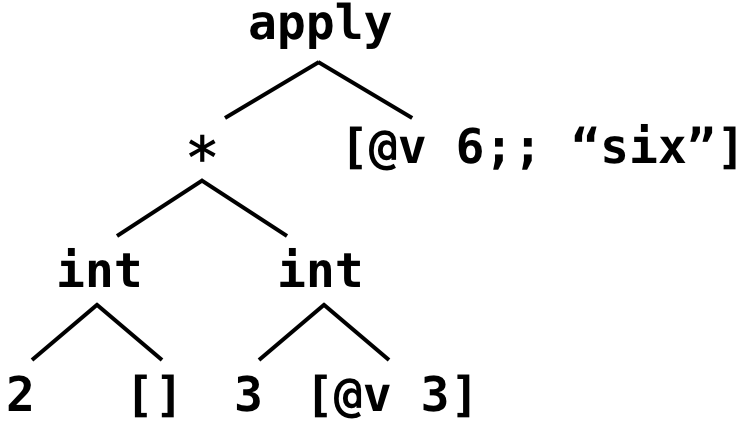
\includegraphics[width=5.2cm, height=3cm]{5/attribute.png}
  \end{center}
  \caption{attribute を含む構文木の例}
  \label{figure:attribute}
\end{figure}

OCaml のプログラムでは、任意の部分式に attribute をつけることができる。式 \texttt{e} に OCaml プログラム \texttt{P} を引数に持つ \texttt{name} という attribute を付けたものは \texttt{e[@name P ]} と書く。例えば \texttt{(2 * 3[@v 3])[@v 6;; "six" ]} という式は大まかには図\ref{figure:attribute}のように構文解析され、ステッパプログラムのように構文木を扱うプログラムの中で attribute の内容を利用することができる。通常の OCaml コンパイラは attribute を無視するので、シンタックスエラー等を起こしてしまう場合を除いて、attribute が付いた式と付いていない式で意味は変わらない。

\begin{figure}
\begin{alltt}
  (* Step 0 *)                              (* Step 0 *)
  (2 * 3) + (5 * 7)[@stepper.redex ]        (2 * 3) + \colorbox{lightgreen}{(5 * 7)}
  (* Step 1 *)                              (* Step 1 *)
  (2 * 3) + 35[@stepper.reduct ]            (2 * 3) + \colorbox{purple}{35}
  (* Step 1 *)                              (* Step 1 *)
  (2 * 3)[@stepper.redex ] + 35             \colorbox{lightgreen}{(2 * 3)} + 35
  (* Step 2 *)                              (* Step 2 *)
  6[@stepper.reduct ] + 35                  \colorbox{purple}{6} + 35
  (* Step 2 *)                              (* Step 2 *)
  (6 + 35)[@stepper.redex ]                 \colorbox{lightgreen}{(6 + 35)}
  (* Step 3 *)                              (* Step 3 *)
  41[@stepper.reduct ]                      \colorbox{purple}{41}
\end{alltt}
\caption{ハイライトのための attribute の利用}
\label{figure:highlight}
\end{figure}

著者らが実装した incremental でないステッパ\cite{FCA19}では、各ステップで簡約が起こっている部分の式をハイライトして示すために attribute を利用している。例えば \texttt{(2 * 3) + (5 * 7)} というプログラムに対する incremental でないステッパの出力は図\ref{figure:highlight}の左の文字列である。インタフェースを受け持つプログラムはこの文字列を受け取り、図\ref{figure:highlight}の右側のように、 attribute が付いた式をハイライトし、さらに attribute を表す文字列を削除した上で表示している。

本研究の incremental なステッパでも、同様の方法で簡約部分のハイライトを行う。本稿ではこれ以降、ステッパの出力文字列中のハイライトのための attribute を省略したり、緑色および紫色のハイライトで現すことがある。

\subsection{プログラムの attribute}
\label{OCamlのattribute-プログラムのattribute}
attribute はプログラム自体にも付けることができる。

OCaml のプログラムは structure item の列であり、structure item には式、変数定義(\texttt{let 変数名 = 式})、型定義、モジュール定義、attribute などの種類がある。structure item の間には \texttt{;;} を書くことで明示的に structure item の境を示すことができる。

attribute の structure item はプログラム中に何度でも書くことができ、名前の重複などに関する制約も無い。また式に付ける attribute と同じく、標準のコンパイラなどはこれを無視するのでプログラムの意味に影響を与えない。

\texttt{name} という名前で OCaml プログラム\texttt{P} を含む attribute の structure item を \texttt{[@@@name P ]} と書く。例えば \texttt{let a = 1 [@@@name1 1;; 2 + 3 ] let b = 2 [@@@name2 ]} というプログラムは、(1)\texttt{a} の定義、(2)\texttt{1} と \texttt{2 + 3} を引数に持つ \texttt{name1} という attribute、(3)\texttt{b} の定義、(4)引数なしの \texttt{name2} という attribute、の4つの structure item のリストとして処理され、それぞれの attribute の内容はステッパが参照することができる。

これを用いると、プログラムに自由に情報を付加することができる。
